\begin{frame}{The Binary Ostensibly-Implicit Tree}
    Рассмотрим еще одну имплицитную структуру в форме \textbf{полного бинарного дерева} для сжатия данных BVH.

    \begin{block}{Хранение дополнительных узлов}
        В MVH есть проблема - постоянный максимум $2N - 1$ узлов, которую мы решали просто дублированием последнего узла
    \end{block}

    \begin{block}{}
        Попробуем хранить \textbf{минимальное число узлов} для объекта, сохраняя гейны от неявно-индексированного дерева
    \end{block}

    \begin{figure}
    \begin{center}
        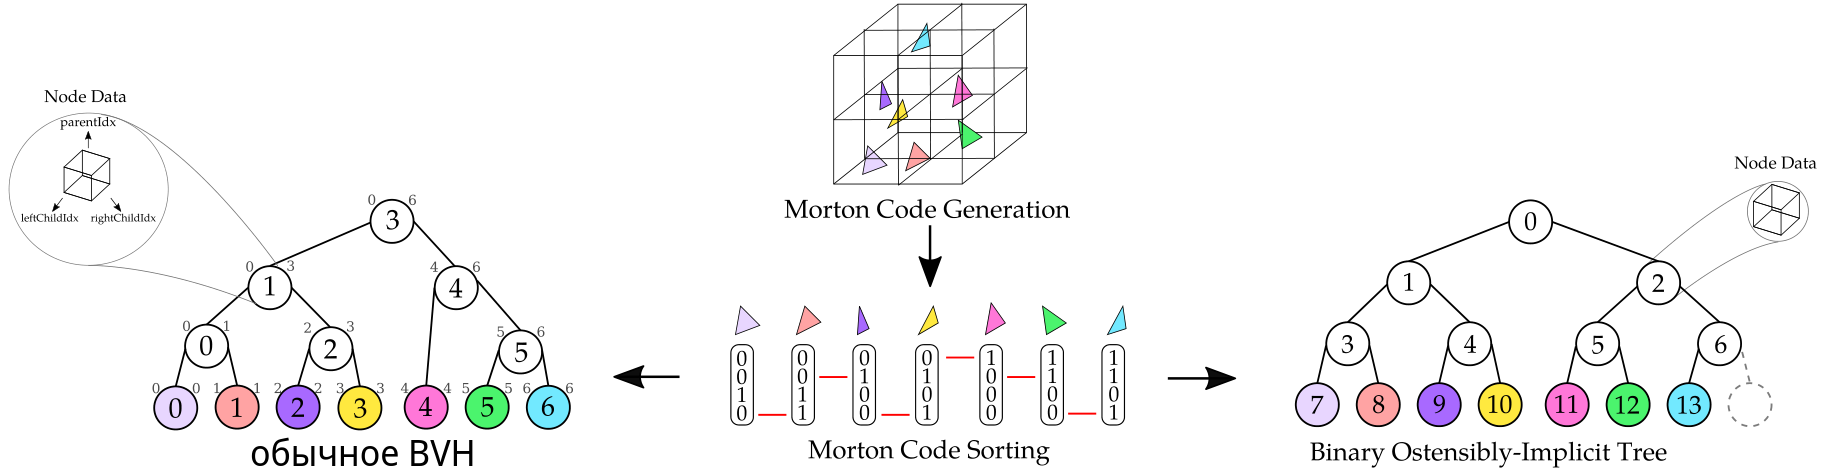
\includegraphics[width=\textwidth]{res/boi.png}
    \end{center}
    \end{figure}

\end{frame}

\begin{frame}[t]{Реальные и виртуальные узлы}
    \framesubtitle{Oi-BVH}
    Лейаут дерева задается параметром $t$ - кол-во примитивов
    \begin{columns}
        \column{0.5\textwidth}
        \begin{block}{Real Nodes}
            \textit{Реальные} узлы содержат только AABB. Нам не нужно хранить ничего более благодаря неявной индексации
        \end{block}
        \begin{block}{Virtual Nodes}
            \textit{Виртуальные} узлы - неиспользованные элементы, когда $t$ не степень двойки.
            Они \textbf{не материализуются в памяти}
        \end{block}
        \column{0.5\textwidth}
        \begin{figure}
            \begin{center}
                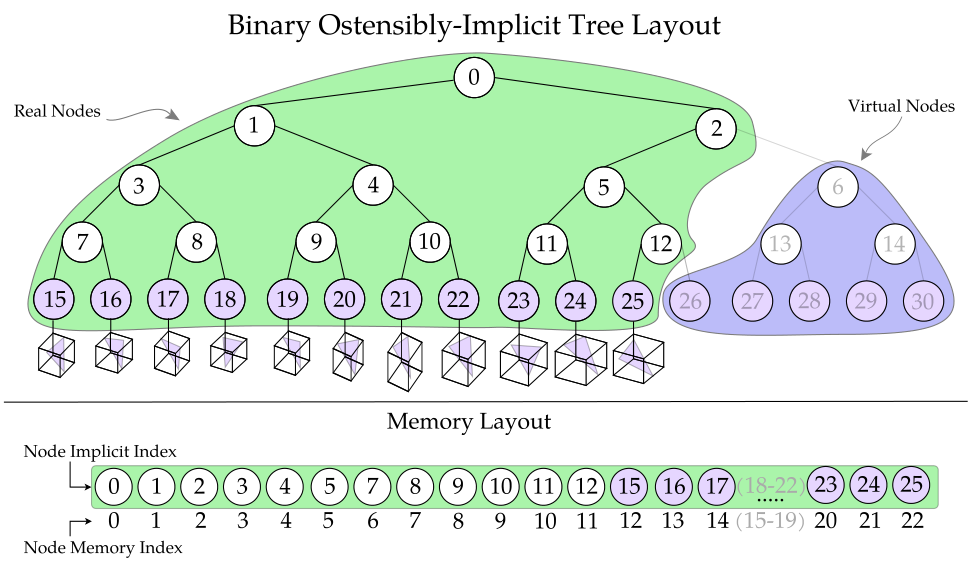
\includegraphics[width=\textwidth]{res/boi_layout.png}
            \end{center}
        \end{figure}
        На всех уровнях дерева виртуальные узлы \textbf{справа}

        Зная кол-во \textit{реальных узлов} на
        уровне можно проверить \textit{виртуальность} узлов.
    \end{columns}

\end{frame}

\begin{frame}[t]{Неявная индексация}
    \framesubtitle{Oi-BVH}
    \begin{itemize}
        \item
            $i$ \textbf{- неявный индекс реального узла}
        \item
            \textbf{Его уровень:} $l_i = \lfloor \log_2 (i + 1) \rfloor, (0 \le l_i \le \bar{l} = \lceil log_2 t \rceil) $
        \item
            \textbf{Кол-во виртуальных узлов на этом уровне:}
            $L_{vl} = \lfloor \frac{L_v}{2^{\bar{l} - l}} \rfloor \equiv L_v \gg (\bar{l} - l)$
        \item
            \textbf{Кол-во виртуальных узлов на этом уровне и выше:}
            $N_{vl} = 2L_{vl} - count\_set\_bits(L_{vl})$
        \item
            \textbf{Индекс узла} $i$ \textbf{в памяти:}
            $i_m = i - N_{vl}, l = l_i - 1$
    \end{itemize}

    \begin{block}{}
        В отличие от \textbf{heap}, где все уровни (кроме, может быть, последнего) заполнены узлами, эта индексация позволяет
        более высоким уровням иметь пустоты. Можно сказать, что такое дерево будет более приближено к оптимальному
    \end{block}
\end{frame}

\begin{frame}[t]{Construction Pipeline}
    \framesubtitle{Oi-BVH}
    \begin{enumerate}
        \setcounter{enumi}{-1}
        \item
            Вычисляем BB для примитивов и присваиваем их к листовым узлам
        \item
            Вычисляем \textbf{Morthon Code} для каждого узла (по расположению центра BB)
        \item
            Сортируем узлы по кодам
        \item
            Строим BVH дерево уровень за уровнем
    \end{enumerate}
    \begin{figure}
        \begin{center}
            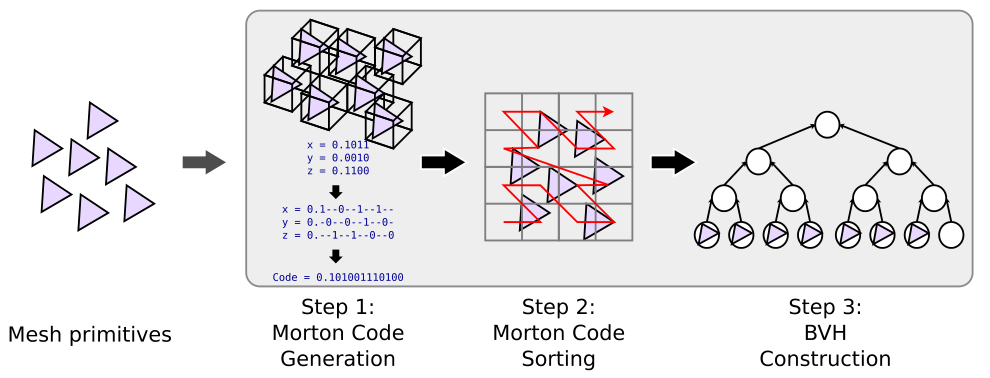
\includegraphics[width=0.9\textwidth]{res/boi_pipeline.png}
        \end{center}
    \end{figure}
\end{frame}

\begin{frame}[fragile]{Алгоритм построения BVH}
    \framesubtitle{Oi-BVH}
    \begin{adjustbox}{width=\textwidth, keepaspectratio}
        \begin{lstlisting}[language=C++,basicstyle=\ttfamily,keywordstyle=\color{blue}]
parallel for each group :
    node_idx = (2^entry_lvl - 1) + global_id

    // mapping treads to nodes of a subtree on the entry lvl
    bboxes = (entry_lvl == leaf_lvl - 1) ? leaf_bboxes : int_bboxes
    l_bbox, r_bbox = get_child_bboxes(bboxes, node_idx, ...)
    write_bbox(int_bboxes, merge(l_bbox, r_bbox), ...)

    // iteratively compute BV at higher lvls
    subtree_root_lvl = entry_lvl - log(group_size)
    lvl = entry_lvl
    while lvl >= subtree_root_lvl:
        node_idx = (2^lvl - 1) + global_id / 2^(entry_lvl - lvl)
        if right_child_is_real and first_tread2reach(node_idx):
            break
        l_bbox, r_bbox = get_child_bboxes(bboxes, node_idx, ...)
        write_bbox(int_bboxes, merge(l_bbox, r_bbox), ...)
        lvl--
        \end{lstlisting}
    \end{adjustbox}

\end{frame}

\begin{frame}{Плюсы и минусы}
    \framesubtitle{Oi-BVH}

    \textbf{Достоинства}:
    \begin{itemize}
        \item
            Шустрый алгоритм построения - 4.5x быстрее LBVH
        \item
            Не нуждается в постобработке для сжатия
        \item
            Дерево хранит только AABB
        \item
            Пространственная локальность узлов (Z-curve)
        \item
            Позволяет иметь пустые узлы на верхних слоях
    \end{itemize}

    \textbf{Недостатки}:
    \begin{itemize}
        \item
            Постоянные проверки на реальность узлов
        \item
            BFS, а значит не кэш-френдли алгоритмы для обхода
        \item
            Сильно страдает от \textit{оторванных} примитивов
        \item
            BVH с повышенной SAH-cost
    \end{itemize}

\end{frame}

